\chapter{Основные теоретические сведения}
Визуализация графа — это графическое представление вершин и ребер графа. Визуализация строится на основе исходного графа, но направлена на получение дополнительных атрибутов вершин и ребер: размера, цвета, координат вершин, толщины и геометрии ребер. Помимо этого, в задачи визуализации входит определение масштаба представления визуализации.

\begin{figure}[h!]
	\centering
	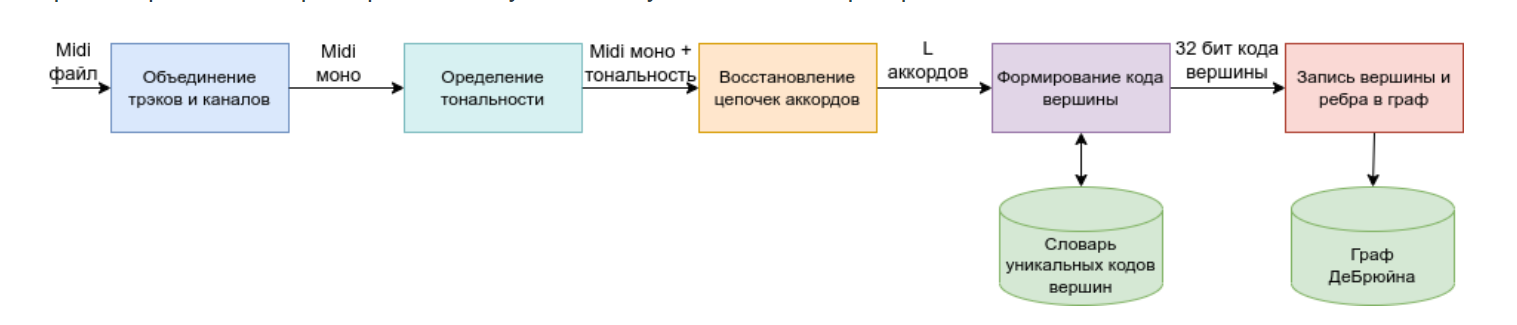
\includegraphics[scale=0.5]{img/1.png} % height
	\caption{"Конвейер генерации музыки. Этап 1 - создание графов де Брюйна"}
	\label{img:test}
\end{figure}

1. Объединение треков и каналов — инструменты исходного midi сводятся в один голос.

2. Определение тональности — используется алгоритм на основе Байесовского классификатора (TemperleyKostkaPayne алгоритм).

3. Восстановление цепочек аккордов — последовательность событий преобразуется в состояния.

4. Формирование кода вершины — каждое состояние кодируется в виде последовательности нот. Для состояния из Словаря уникальных кодов вершин получается уникальный ключ вершины.

5. Запись вершины и ребра в граф - ключ вершины добавляется в граф деБрюйна и соединяется ребром с предыдущей вершиной.

6. Граф ДеБрюйна передается в gpc и выполняется его анализ алгоритмом Ньюмана (выделение сообществ).

7. Рендер графа передается в хост-подсистему для визуализации.
\chapter{Экспериментальная часть}

\section{Индивидуальное задание}

Выбрать музыкальное произведение различных композиторов и жанров. Произведение должно быть доступно в формате midi. Используя код Проекта 6 получить по визуализации для музыкального произведения. С помощью приложением стилизация графов.

\section{Результаты}

\begin{figure}[h!]
	\centering
	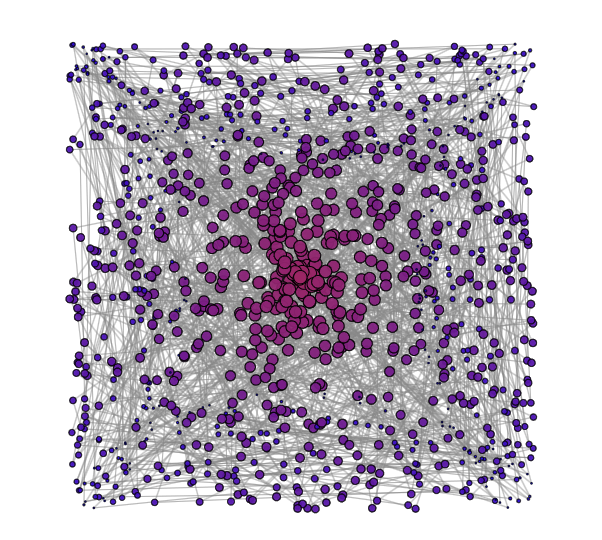
\includegraphics[scale=1]{img/sem2.png} % height
	\caption{"Визуализация на основе модулярности Ньюмана"}
	\label{img:sem2}
\end{figure}

\begin{figure}[h!]
	\centering
	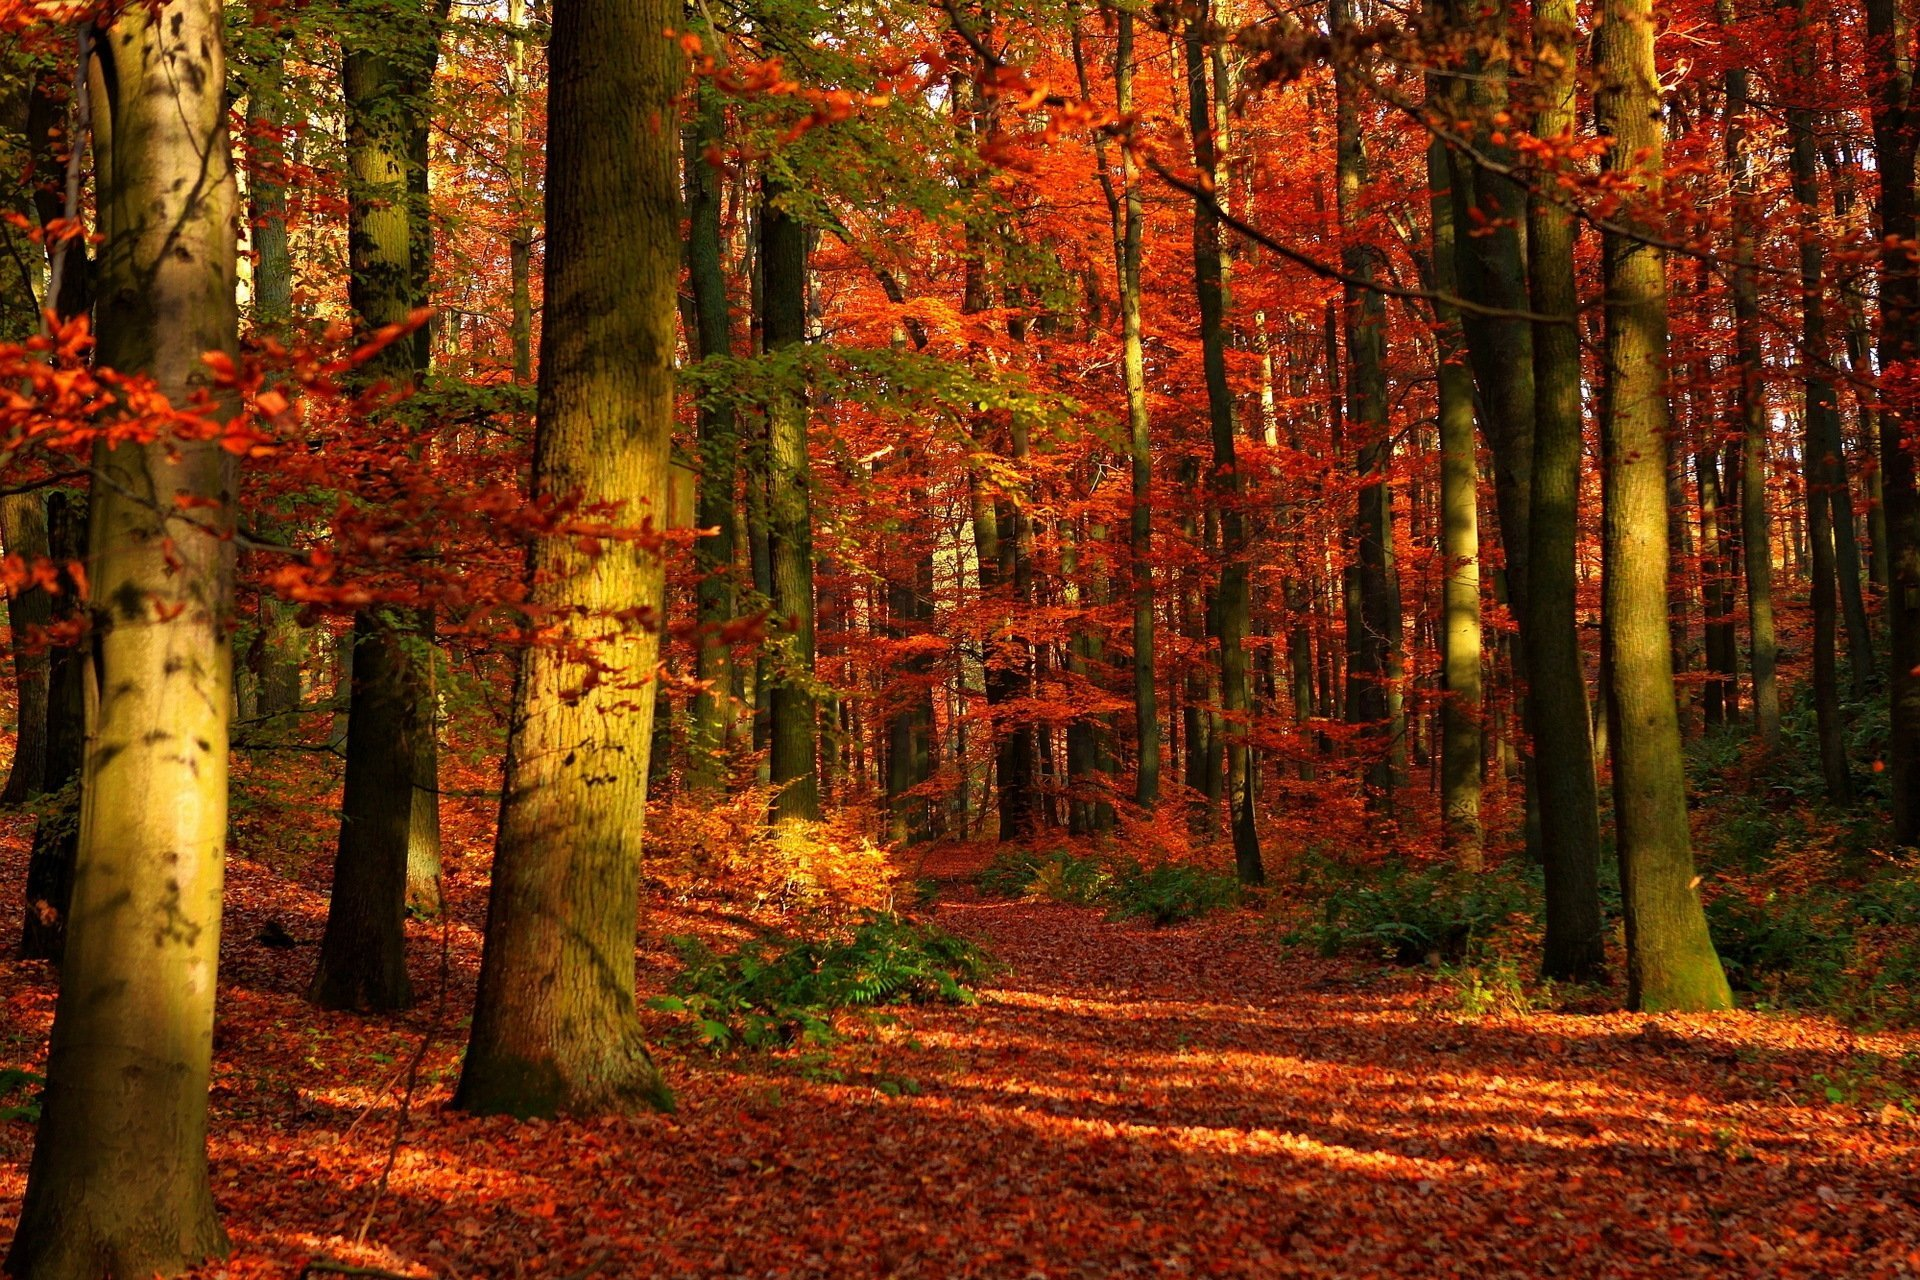
\includegraphics[scale=0.3]{img/styled.jpg} % height
	\caption{"Изображение леса осенью"}
	\label{img:styled}
\end{figure} 

\begin{figure}[h!]
	\centering
	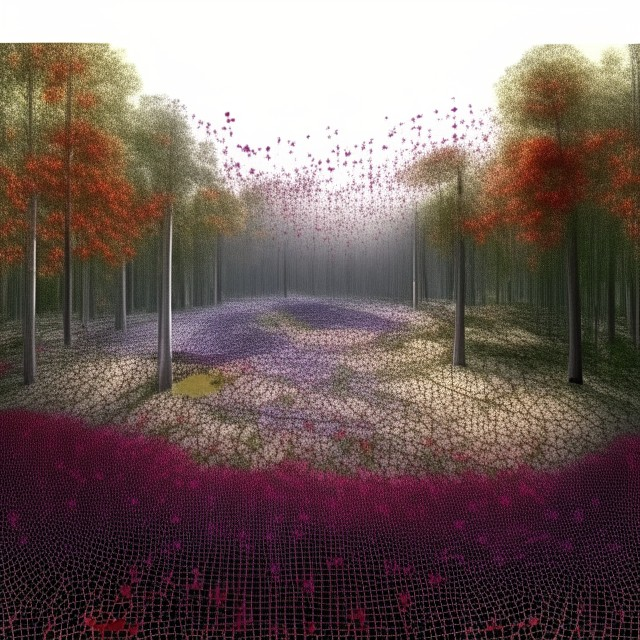
\includegraphics[scale=0.7]{img/result.jpeg} % height
	\caption{"Изображение после стилизации "}
	\label{img:result}
\end{figure} 
\clearpage
\section{Вывод}
В ходе практикума было проведено ознакомление с вариантами представления  графов в виде объединения структур языка C/C++, изучены и применены на практике примеры решения некоторых задач на графах.
По индивидуальному варианту была разработана программа хост-подсистемы и программного ядра 
sw\_kernel, выполняющего обработку и визуализацию графов